%-------------------------
% Rover Resume - Fancy Template
% Link: https://github.com/subidit/rover-resume
%------------------------

\documentclass[11pt]{article}

\usepackage[T1]{fontenc}
\usepackage{inter} % https://tug.org/FontCatalogue/
\renewcommand*\familydefault{\sfdefault}
\usepackage{graphicx}

\usepackage{geometry}
\geometry{
a4paper,
top=1.8cm,
bottom=1in,
left=2.5cm,
right=2.5cm
}

\setcounter{secnumdepth}{0} % remove section numbering
%\pdfgentounicode=1 % make ATS friendly

\usepackage{enumitem}
\setlist[itemize]{
    noitemsep,
    left=0pt..1.5em
}
\setlist[description]{itemsep=0pt}
\setlist[enumerate]{align=left}

\usepackage[dvipsnames]{xcolor}
% \usepackage[dvipsnames, svgnames, x11names]{xcolor} 
% \usepackage[dvipsnames]{xcolor} % xcolor.pdf Sec.4 Colors by Name
\colorlet{icnclr}{gray}
% \colorlet [⟨type⟩]{⟨name⟩}[⟨num model⟩]{⟨color ⟩}
% \definecolor[⟨type⟩]{⟨name⟩}{⟨model-list⟩}{⟨spec-list⟩}


\usepackage{titlesec}
% \titlespacing{command}{left spacing}{before spacing}{after spacing}[right]
% \titlespacing{\section}{0pt}{*3}{*1}
\titlespacing{\subsection}{0pt}{*0}{*0}
\titlespacing{\subsubsection}{0pt}{*0}{*0}
% \titleformat{<command>}[<shape>]{<format>}{<label>}{<sec>}{<before-code>}[<after-code>]  
\titleformat{\section}{\color{Sepia}\large\fontseries{black}\selectfont\uppercase}{}{}{\ruleafter}[\global\RemVStrue]
\titleformat{\subsection}{\large\fontseries{semibold}\selectfont}{}{}{\rvs}
\titleformat{\subsubsection}{\large\fontseries{medium}\selectfont}{}{}{}

\usepackage{xhfill} 
\newcommand\ruleafter[1]{#1~\xrfill[.5ex]{1pt}[gray]} % add rule after title in .5 x-height 

\newif\ifRemVS % remove vspace between \section & \subsection
\newcommand{\rvs}{
    \ifRemVS
        \vspace{-1.5ex}
    \fi
    \global\RemVSfalse
}


\usepackage{fontawesome5}

\usepackage[bookmarks=false]{hyperref} % [imp!]
\hypersetup{ % https://en.wikibooks.org/wiki/LaTeX/Hyperlinks
    colorlinks=true,
    urlcolor=Sepia,
    pdftitle={My Resume}}

\usepackage[page]{totalcount}
\usepackage{fancyhdr}
\pagestyle{fancy}
\renewcommand{\headrulewidth}{0pt}	
\fancyhf{}							
\cfoot{\color{darkgray} Alessio Rovere CV (ENG) -- Page \thepage{} of \totalpages}


\usepackage[backend=biber,style=apa,sorting=ydnt,uniquename=false,isbn=false,maxbibnames=99,url=false,giveninits=true,eprint=false]{biblatex}
\AtEveryBibitem{\clearfield{note}}
\addbibresource{sample.bib}


\begin{document}
% ---------- ENGLISH ----------------------
\newpage
\begin{center}
    {\fontsize{36}{36}\selectfont\interthin Alessio \interheavy Rovere} \\ \bigskip
    {\fontsize{14}{14}\selectfont\interthin Curriculum Vitae - English version}\\ \bigskip
    {\color{icnclr}\faEnvelope[regular]} \href{mailto:alessio.rovere@unive.it}{alessio.rovere@unive.it}
\end{center}

\section{Academic Qualifications}
{\normalfont My academic studies took place at the University of Genoa, Italy, renowned for its excellence in marine environmental sciences and geosciences. I won two degree awards, one for my bachelor's thesis and one for my master's thesis. During my Ph.D., I participated in several research stays abroad and earned the \textit{"European Ph.D. Label"}.} \\
\bigskip
\subsection{Università degli Studi di Genova $|$ {\normalfont\textit{Ph.D. in Marine Sciences}} \hfill 06/2011}
{\footnotesize My Ph.D. research received the recognition \textit{"European Ph.D. label"}. As such, it required at least six months of research abroad, thesis evaluation by two professors from different European countries, the participation of at least one committee member from a European country other than Italy, and the defense of the thesis in an official EU language other than Italian. My main supervisor was Prof. Marco Firpo. \\
\textbf{Thesis}: \textit{Rocky Coasts in the Ligurian Sea: Morphology, Evolution, and Management Aspects}.\\ 
\textbf{Periods abroad during Ph.D.}: University of Western Australia, AU (2010, 1 month); Brunel University, UK (2010, 4 months); University of the Aegean, GR (2010, 17 days); University of the Aegean, GR (2009, 1 month).}
\bigskip

\subsection{Università degli Studi di Genova $|$ {\normalfont\textit{MSc in Marine Environmental Sciences}} \hfill 07/2006}
{\footnotesize I completed a two-year master's degree in Marine Environmental Sciences, during which I received an ERASMUS scholarship. I graduated with a final grade of 110/110. My main supervisors were Prof. Marco Firpo and Prof. Carlo Nike Bianchi. \\
\textbf{Thesis}: \textit{Cartography and Geomorphology of the Seabed in the Bergeggi Marine Protected Area (SV)} (thesis written in Italian).\\
\textbf{ERASMUS Scholarship}: Universidad de Las Palmas de Gran Canaria, ES (2004, 3 months, 18 days).\\
\textbf{Degree Award}: "Premio Parchi Cum Laude", Liguria Region (2010), second prize ex-aequo.}
\bigskip

\subsection{Università degli Studi di Genova $|$ {\normalfont\textit{BSc in Environmental Sciences}} \hfill 02/2004}
{\footnotesize I completed a three-year undergraduate course in Environmental Sciences, graduating with the highest marks, 110/110. I conducted my thesis under the guidance of Prof. Carlo Nike Bianchi. \\
\textbf{Thesis}: \textit{Geological and Geomorphological Features of the Seabed around Bergeggi Island related to the Establishment of the Marine Protected Area} (thesis written in Italian).\\
\textbf{Degree Award}: "Prix Alain Vatrican 2003 (RAMOGE, Monaco)" first prize ex-aequo.}
\newpage

\section{Academic Positions}
{\normalfont After completing my Ph.D., my academic career has primarily been international. I spent two years in the United States at Columbia University, which is ranked 17th in the 2024 World University Rankings by THE, followed by eight years at Universität Bremen, recognized as a German \textit{"University of Excellence"}. I returned to Italy in 2021. Since March 2014, just two years and nine months post-Ph.D., I have independently led my own research group.}\\
\bigskip
\subsection{Università Ca' Foscari Venezia $|$ {\normalfont\textit{Full Professor}} \hfill 11/2024 - Present}
{\footnotesize As a Full Professor, my responsibilities encompass teaching, research, and faculty administration, steering decisions on the Department and University strategy.}
\bigskip
\subsection{Università Ca' Foscari Venezia $|$ {\normalfont\textit{Associate Professor}} \hfill 11/2021 - 11/2024}
{\footnotesize My position As Associate Professor at Ca' Foscari was made through a direct appointment following a positive evaluation by the Italian Ministry for University and Research (prot. n. 11888, 4.09.2021), pursuant to Article 1, Paragraph 9 of Law n. 230/2005.}
\bigskip

\subsection{Universität Bremen $|$ {\normalfont\textit{Professor}} \hfill 04/2020 - 10/2021}
{\footnotesize Alongside my role as a \textit{"Research group leader"}, I was granted the title of \textit{"Professor"} in accordance with Article 17 of the Higher Education Act of the State of Bremen.}
\bigskip

\subsection{Universität Bremen $|$ {\normalfont\textit{Research group leader}} \hfill 03/2019 - 10/2021}
{\footnotesize As a tenured \textit{Research group leader} at MARUM (Center for Marine Environmental Sciences), affiliated with the University of Bremen, I led the research group \textit{"Sea Level and Coastal Changes"}. My duties included spearheading research initiatives and teaching at the University of Bremen, with a primary focus on advancing research in coastal geosciences.}
\bigskip

\subsection{Universität Bremen and Leibniz ZMT $|$ {\normalfont\textit{Young Group Leader}} \hfill 03/2014 - 02/2019}
{\footnotesize As a tenure-track \textit{"Young Research Group Leader"} at MARUM (Center for Marine Environmental Sciences) and the Leibniz Centre for Tropical Marine Research (ZMT), I founded and led the research group \textit{"Sea Level and Coastal Changes".} My role involved establishing leadership in the field, spearheading research initiatives, managing grants and securing funding. I also engaged in teaching activities at the University of Bremen.}
\bigskip

\subsection{Columbia University $|$ {\normalfont\textit{Postdoctoral Researcher}} \hfill 02/2012 - 02/2014}
{\footnotesize As a postdoctoral researcher at the Lamont-Doherty Earth Observatory of Columbia University, I conducted research within the project \textit{"PLIOcene MAXimum sea level (PLIOMAX)"} funded by the US National Science Foundation. I worked under the guidance of Prof. Maureen E. Raymo.}
\bigskip

\section{Technological Transfer}
{\normalfont During my Ph.D. at the University of Genoa, I co-founded SeaMap srl, an environmental consulting company, in collaboration with six partners. The company secured initial funding through a consortium started by the University of Genoa (UNITI) and was later recognized as a university spin-off. As the sole administrator, I managed operations until its closure. In 2011, SeaMap received the \textit{"Italy of Innovators"} award from the \textit{"Agency for the Dissemination of Technologies for Innovation - Presidency of the Council of Ministers"}.}\\
\bigskip

\subsection{SeaMap srl $|$ {\normalfont\textit{Director}} \hfill 10/2010 - 12/2016}
{\footnotesize Serving as the Director (Amministratore Unico), I led both the technical and administrative aspects of commercial projects, managing research and development activities. I was responsible for the management of startup funds and effectively managed around 150,000 euros (excluding VAT) in commercial and research and development projects .}

\section{Other Academic Positions}
{\normalfont In addition to my principal academic work positions, I have held several appointments as adjunct faculty.}\\
\bigskip

\subsection{Universität Bremen $|$ {\normalfont\textit{Honorary Professor}} \hfill 03/2024 - Present}
{\footnotesize I have been conferred the title of Honorary Professor by a committee nominated by the University of Bremen. This appointment involves active participation in teaching and collaborative research activities.}
\bigskip

\subsection{MARUM - Universität Bremen $|$ {\normalfont\textit{External Member}} \hfill 10/2021 - Present}
{\footnotesize As an external member at MARUM, I am expected to actively engage in research activities within the designated cluster, dedicating time to project meetings, participating in thesis committees, and fulfilling similar commitments.}
\bigskip

\subsection{LDEO - Columbia University $|$ {\normalfont\textit{Adjunct Research Scientist}} \hfill 04/2014 - 08/2021}
{\footnotesize As an adjunct research scientist at LDEO, my role involved engaging in research activities at the Observatory while maintaining my primary affiliation with another institution.}

\section{University Service}
%===============
{\normalfont As an Associate Professor at Ca' Foscari University, I have undertaken various responsibilities in overseeing and managing both teaching and research activities.}\\
%============
\bigskip
\subsection{Università Ca' Foscari Venezia  $|$ {\normalfont\textit{Teaching Coordinator}} \hfill 04/2024 - Present}
{\footnotesize As the Coordinator of the educational college, appointed by the DAIS Department Council of Ca' Foscari on 26.03.2024, for Environmental Sciences, I manage the supervision and implementation of the Study Program, including its continuous review. I promote the Quality Assurance process, aligning it with the strategic objectives of the University and the Department, and ensure compliance with the guidelines of ANVUR (National Agency for the Evaluation of the University and Research Systems).}

\bigskip

\subsection{Università Ca' Foscari Venezia $|$ {\normalfont\textit{Ph.D. Program Board}} \hfill 05/2023 - Present}
{\footnotesize I am a member of the Ph.D. Program Board (Collegio di dottorato) for the \textit{"Doctoral of National Interest in Polar Sciences"} at Ca' Foscari University of Venice.}
\bigskip

\subsection{Università Ca' Foscari Venezia $|$ {\normalfont\textit{Ph.D. Program Board}} \hfill 05/2022 - Present}
{\footnotesize I serve on the Ph.D. Program Board (Collegio di dottorato) in \textit{"Polar Sciences"} at Ca' Foscari University of Venice.}
\bigskip

\subsection{Università Ca' Foscari Venezia  $|$ {\normalfont\textit{ERASMUS Commission}} \hfill 12/2022 - Present}
{\footnotesize I am a member of the \textit{"Erasmus Commission for Environmental Sciences"} (nominated by the Ca' Foscari DAIS Department Council on 13.12.2022). In this capacity, I assist in overseeing ERASMUS scholarship requests and contribute to the internationalization of our student body.}
\bigskip

\subsection{Università Ca' Foscari Venezia  $|$ {\normalfont\textit{ERC Board}} \hfill 09/2022 - Present}
{\footnotesize As a member of the \textit{"Ca' Foscari ERC Board"} (appointed by Ca' Foscari Rector’s Decree 815/2022), I evaluate applications and act as a liaison between my Department and Principal Investigators of ERC grants who initially selected a different Italian or foreign institution as their Host Institution but intend to transfer to Ca' Foscari. I actively seek out talented researchers and initiate contact with them.}
\bigskip

\subsection{Università Ca' Foscari Venezia  $|$ {\normalfont\textit{ESA Lab}} \hfill 2022 - Present}
{\footnotesize I am a member of the \textit{"ESA Lab@CaFoscari"} Steering Committee (Ca' Foscari and European Space Agency), which promotes, coordinates, and supports research activities, scientific collaborations, teaching initiatives, and scientific events related to space data and related research.}

\newpage
\section{Service for Research Organisations}
%===============
{\normalfont I am an active member of the international scientific community, specializing in paleo sea-level changes and broader coastal processes.}\\
%============
\bigskip
\subsection{INQUA $|$ {\normalfont\textit{INQUA CMP Commission President}} \hfill 2023 - Present}
{\footnotesize As President of the Coastal and Marine Processes Commission of the International Union for Quaternary Science (INQUA), I guide strategic decisions and oversee funding applications for conferences and workshops.}
\bigskip

\subsection{SCAR-INSTANT $|$ {\normalfont\textit{Steering Committee}} \hfill 2022 - Present}
{\footnotesize As a member of the Steering Committee for the \textit{"Instabilities and Thresholds in Antarctica"} (INSTANT) project under the \textit{"Scientific Committee on Antarctic Research"} (SCAR), I contribute to steering decisions on scientific directions and serve in an advisory role.}
\bigskip

\subsection{PALSEA $|$ {\normalfont\textit{Co-Leader}} \hfill 2018 - 2023}
{\footnotesize I served as co-leader (with three other scientists) of the PALSEA (PALeo constraints on SEA level rise) project, funded by the International Union of Quaternary Sciences (INQUA) and Past Global Changes (PAGES). I directed strategic decisions on the project's scientific focus, promoted activities to expand its scope, and handled travel funding applications from early career researchers.}
\bigskip

\subsection{MPA "Cinque Terre" $|$ {\normalfont\textit{Scientific Committee Member}} \hfill 06/2021 - Present}
{\footnotesize As a member of the Scientific Committee of the Marine Protected Area (MPA) \textit{"Cinque Terre"}, I contribute to overseeing scientific activities within the MPA and provide guidance on technical and scientific issues related to its management.}
\bigskip

\subsection{MEDFLOOD/MOPP $|$ {\normalfont\textit{Co-Leader}} \hfill 2012 - 2018}
{\footnotesize I served as co-leader (with three other scientists) of the MEDFLOOD and MOPP projects, funded by the International Union for Quaternary Science (INQUA) to support yearly workshops and training schools on Mediterranean sea-level science. I directed strategic decisions on the project's scientific focus, promoted activities to expand its scope, and handled travel funding applications from early career researchers.}

\section{Scientific Committees of conferences}
{\normalfont Throughout my career, I have actively organized meetings and proposed sessions for international conferences. Below is a list of conferences and workshops where I served on the organizing committee, or took on the role of session organizer, convener, or chair.}\\

\bigskip
{\normalfont 
\subsection{Member of scientific and organisation committees}}
{\footnotesize
\begin{description}
  \item [2022] PALSEA annual meeting, Singapore.
  \item [2021] Webinar series by PALSEA, WCRP (sea level), IAG, and SERCE.
  \item [2020] "PALSEA Express" online workshop.
  \item [2019] CoChE Summer school. Coastal Changes and Evolution. Oristano (IT).
  \item [2019] PALSEA workshop "Using ecological and chronological data to improve proxy-based paleo sea level reconstructions", Dublin (IE).
  \item [2017] PALSEA-QUIGS meeting on “Climate, ice sheets and sea level during past interglacial periods”. Galloway, New Jersey (USA)
  \item [2012] Annual MEDFLOOD workshop, Rome (IT).
  \item [2014] Annual MEDFLOOD workshop, Haifa (IL).
  \item [2016] Annual MEDFLOOD workshop, Bremen (DE)
  \item [2013] Organizer of the bi-weekly seminar at Lamont Doherty Earth Observatory, Biology and Paleo Environment Division
  \item \end{description}}

{\normalfont 
\subsection{Session organiser, convener or chair}}
{\footnotesize
\begin{description}
  \item [2023] Rome INQUA conference. Session 89: "Cenozoic sea-level indicators and ice sheet constraints to global sea-level change".
  \item [2022] PAGES Open Science Meeting. Session: "Last Interglacial".
  \item [2019] American Geophysical Union 2019. Session PP23A: "Centennial Session: One Hundred Years of Ice Sheet and Sea Level Science".
  \item [2017] GeoBremen conference. Session: "Coastal depositional environments \& processes"
  \item [2015] American Geophysical Union 2015. Session PP11E: "Sea Levels and Ice Sheets during Past Warm Periods: Looking to the Past to Understand the Future".
  \item \end{description}}

\section{Other Relevant Scientific Roles}
\subsection{IPCC AR6 $|$ {\normalfont\textit{Contributing Author}} \hfill 2022}
{\footnotesize I was a contributing author for the Intergovernmental Panel on Climate Change (IPCC) Sixth Assessment Report (AR6), contributing to Chapters 2 and 9 of Working Group 1. As a contributing author, I provided technical information, including text, graphs, and data, for integration into the draft sections.}

\section{Invited seminars and talks}
{\normalfont In addition to my teaching responsibilities, I am frequently invited to present my research at university seminars and international conferences. Below is a list of the most significant talks I have given over the years.}\\
{\footnotesize 
\begin{description}
  \item [2023] University of Genoa (IT).
  \item [2023] QUIGS workshop (Online).
  \item [2022] ECORD Summer School 2022 (DE).
  \item [2021] Ca’ Foscari University of Venice (IT).
  \item [2019] PAGES ECN grant-writing workshop, Prague (CZ).
  \item [2018] Ca’ Foscari University of Venice (IT).
  \item [2018] Durham University (UK).
  \item [2018] CEREGE, Université Aix-Marseille (FR).
  \item [2017] Bonn University (DE).
  \item [2017] University of Cambridge (UK).
  \item [2017] Université de Bretagne Occidentale, Brest (FR).
  \item [2017] University of Genoa (IT).
  \item [2016] American Geophysical Union, San Francisco (USA).
  \item [2015] LDEO, Columbia University (USA).
  \item [2013] University of Bremen (DE).
  \item [2012] Rice University, Houston (USA).
  \item [2008] Université du Sud Toulon-Var (FR).
  \item \end{description}}
\newpage
\section{Editorial Roles}
{\normalfont Throughout my career, I have served in various editorial roles.}\\

\bigskip

\subsection{Earth System Science Data $|$ {\normalfont\textit{Editor}} \hfill 2022 - Present}
{\footnotesize I serve as an editor for \textit{Earth System Science Data}, an open-access journal published by Copernicus. The journal has a 2022 impact factor of 11.4. In this role, I have edited 15 manuscripts.}
\bigskip

\subsection{Climate of the Past $|$ {\normalfont\textit{Editor}} \hfill 2022 - Present}
{\footnotesize I serve as an editor for \textit{Climate of the Past}, an open-access journal published by Copernicus. The journal has a 2022 impact factor of 4.3. In this role, I have edited 21 manuscripts.}
\bigskip

\subsection{UAVs in Environmental Sciences $|$ {\normalfont\textit{Book Editor}} \hfill 2019 - 2022}
{\footnotesize I was one of the editors for the open-access textbook \textit{"UAVs in Environmental Sciences"}, published by Wissenschaftliche Buchgesellschaft (WBG).}
\bigskip

\subsection{Earth System Science Data $|$ {\normalfont\textit{Special Issue Editor}} \hfill 2019 - 2022}
{\footnotesize I was an editor for the \textit{Earth System Science Data} Special Issue titled \textit{"The World Atlas of Last Interglacial Shorelines"}.}
\bigskip

\subsection{Quaternary Science Reviews $|$ {\normalfont\textit{Special Issue Editor}} \hfill 2017 - 2018}
{\footnotesize I was an editor for the \textit{Quaternary Science Reviews} Special Issue titled \textit{"Inception of a Global Atlas of Sea Levels since the Last Glacial Maximum"}. Quaternary Science Reviews is a journal published by Elsevier and has a 2022 impact factor of 4.}
\bigskip

\subsection{Alpine and Mediterranean Quaternary $|$ {\normalfont\textit{Editor}} \hfill 2013 - 2017}
{\footnotesize I was an editor for \textit{Alpine and Mediterranean Quaternary}, the journal of the Italian Association for Quaternary Studies (AIQUA).}
\bigskip

\subsection{Quaternary Perspectives $|$ {\normalfont\textit{Editor}} \hfill 2013 - 2014}
{\footnotesize I was an editor for \textit{Quaternary Perspectives}, the newsletter of INQUA, the International Union for Quaternary Sciences.}

\section{Reviewer Roles}
{\normalfont Throughout my career, I have served as a reviewer for several manuscripts and proposals.}\\

\bigskip

\subsection{Various Journals $|$ {\normalfont\textit{Manuscript Reviewer}} \hfill Since 2021}
{\footnotesize I have reviewed nearly 70 manuscripts submitted to international journals, including \textit{Nature}, \textit{Nature Geoscience}, and \textit{Nature Communications}.}
\bigskip

\subsection{Various Funding Agencies $|$ {\normalfont\textit{Proposal Reviewer}} \hfill Since 2021}
{\footnotesize I have reviewed research proposals for various funding agencies, including the \textit{Swiss Science Foundation}, \textit{Humboldt Foundation}, \textit{Israel Science Foundation}, \textit{The Petroleum Research Fund (American Chemical Society)}, University of Singapore, and \textit{National Geographic Society}.}

\newpage

\section{Teaching}
{\normalfont I have been active in teaching at several universities, both in Italy and abroad. Hereafter, a list of the courses I gave over the years. I include overall course evaluations for all courses and years for which they are available.}\\

\bigskip
\subsection{Università Ca' Foscari Venezia (MSc) $|$ {\normalfont\textit{Coastal geological processes and risks}}}
{\footnotesize This course is part of the MSc program in Environmental Sciences, curriculum \textit{"Natural capital and ecosystem services"}. It offers 6 ECTS credits, amounting to a total of 48 hours. The course was taught in the academic years 2023/2024 and (under a slightly different name but with the same content) in 2022/2023.\\
\textbf{Students evaluations}: 2022/2023: 9.55/10 (for both lectures and laboratory).}
\bigskip

\subsection{Università Ca' Foscari Venezia (BSc) $|$ {\normalfont\textit{Physical geography and geomorphology}}}
{\footnotesize This course is part of the BSc program in Environmental Sciences (Subject: GEO/04). It offers 6 ECTS credits, amounting to a total of 48 hours. The course was taught in the academic years 2023/2024 and (under different names but with the same content) in 2022/2023 and 2021/2022 (this year the course was 6 credits, but 60 hours).\\
\textbf{Students evaluations}:
2021/2022: 8.88/10 (lectures) - 8.74/10 (laboratory) $|$ 2022/2023: 8.40/10 (lectures) - 8.03/10 (laboratory).}
\bigskip

\subsection{Universität Bremen (BSc) $|$ {\normalfont\textit{Clastic sedimentology: coastal and shelf dynamics}}}
{\footnotesize This was a course in the BSc program in Geosciences. The entire course is 2 SWS (Semesterwochenstunden), and was split between three teachers. I usually taught three 2-hour lectures in this course, and supervised part of the exams. The course was held from 2018 to 2021.}
\bigskip

\subsection{Università degli Studi di Genova (MSc) $|$ {\normalfont\textit{ERASMUS teaching mobility}}}
{\footnotesize In 2018, I taught 8 hours as part of a teaching exchange between the University of Bremen and the Engineering department (DITEN) at the University of Genoa.}
\bigskip

\subsection{Universität Bremen (Ph.D.) $|$ {\normalfont\textit{Paleo sea level changes}}}
{\footnotesize I taught an 8-hour course titled "Paleo Sea Level Changes: Eustasy, Tectonics, Isostasy" at the Bremen International Graduate School for Marine Sciences - GLOMAR. The course, under slightly different titles but with similar content, was held in 2018, 2016, and 2014.}
\bigskip

\subsection{Universität Bremen (BSc) $|$ {\normalfont\textit{Geographic Information Systems}}}
{\footnotesize This was a course in the BSc program in Geosciences. The entire course is 3 SWS (Semesterwochenstunden), and I co-led the course with another colleague. The course was held in 2017 and 2020. 
\textbf{Students evaluations}: 2017: 1.81 ± 0.68 (where 1= Very good and 5 = Insufficient)}
\bigskip

\subsection{Universität Bremen (BSc) $|$ {\normalfont\textit{Marine Geological Project}}}
{\footnotesize This was a field course held in 2017 within the BSc program in Geosciences, to which I participated as assistant teacher. The course lasted three days, and was held on the island of Helgoland (Northern Germany).}
\bigskip

\subsection{Universität Bremen (MSc) $|$ {\normalfont\textit{Field course Coastal Changes}}}
{\footnotesize This was a field course I led in the MSc program in Marine Geosciences, coordinating two other instructors. This one-week course, held in Italy, was organised as a practical field study and took place in 2017, 2018, and 2019.
\textbf{Students evaluations}: 2018: 1.21 ± 0.43 (where 1= Very good and 5 = Insufficient)}
\bigskip

\subsection{Universität Bremen (BSc) $|$ {\normalfont\textit{Field course carbonate sedimentology}}}
{\footnotesize This was a field course held in 2014 within the BSc program in Geosciences, to which I participated as assistant teacher. The course lasted five days, and was held on the island of Mallorca (Spain).}
\bigskip

\subsection{Università degli Studi di Genova $|$ {\normalfont\textit{Seminars as teaching assistant}}}
{\footnotesize During my masters and Ph.D. at the University of Genoa, I contributed to teaching activities within master and Ph.D. courses. These are listed below.}
{\footnotesize 
\begin{description}
  \item [2011] Use of GIS in the assessment of coastal and marine landscapes (MSc, 6 hours)
  \item [2011] Geomorphology in marine environmental sciences (Ph.D, 6 hours)
  \item [2008] Geomorphological heritage in Marine Protected Areas (MSc, 2 hours)
  \item [2007] Geomorphological heritage in Marine Protected Areas (MSc, 2 hours)
  \item [2005] Seafloor characterisation of Arguineguin, Gran Canary, Spain (BSc, 2 hours)
  \item [2005] Geomorphological and sedimentological outlines of the future MPA of Bergeggi (BSc, 2 hours)
  \item [2005] Seafloor characterisation of Arguineguin, Gran Canary, Spain (BSc, 2 hours)
\end{description}
}

\section{Mentoring of postdoctoral researchers}
{\normalfont Since establishing my own research group at the University of Bremen, I have mentored nine postdoctoral researchers. This group includes both current and former researchers who, upon leaving my team, have successfully transitioned to other academic positions or into industry roles.}\\
\subsubsection{Dr. Ciro Cerrone $|$ {\normalfont\textit{Università Ca' Foscari Venezia}} \hfill 2023 - Present}
{\footnotesize 
\begin{description}
  \item [Research Topic] Last Interglacial sea level changes in South America, Atlantic Ocean. 
\end{description}
}
\smallskip

\subsubsection{Dr. Silas Dean $|$ {\normalfont\textit{Università Ca' Foscari Venezia}}\hfill 2022 - Present}
{\footnotesize 
\begin{description}
  \item [Research Topic] Last Interglacial sea level changes on the US East Coast. 
\end{description}
}
\smallskip
\subsubsection{Dr. Denovan Chauveau $|$ {\normalfont\textit{Università Ca' Foscari Venezia}}\hfill 2022 - Present}
{\footnotesize 
\begin{description}
  \item [Research Topic] Last-Interglacial sea-level oscillations from stratigraphic forward models on coral reefs. 
\end{description}
}

\smallskip
\subsubsection{Dr. Nikos Georgiou $|$ {\normalfont\textit{Università Ca' Foscari Venezia}}\hfill 2022 - Present}
{\footnotesize 
\begin{description}
  \item [Research Topic] Extreme waves in the Last Interglacial and associated coastal landforms. 
\end{description}
}
\smallskip
\subsubsection{Dr. Patrick Boyden $|$ {\normalfont\textit{Universität Bremen}}\hfill 2022 - Present}
{\footnotesize 
\begin{description}
  \item [Research Topic] Ecology of fossil reefs on Aruba, Curacao and Bonaire. 
\end{description}
}

\smallskip
\subsubsection{Dr. Deirdre D. Ryan $|$ {\normalfont\textit{Universität Bremen}}\hfill 2018-2021}
{\footnotesize 
\begin{description}
  \item [Research Topic] Morphology and dating of fossil beach ridges in Patagonia, Argentina. 
  \item [Current position] Environmental Scientist - San Francisco Bay Regional Water Quality Control Board. 
\end{description}
}

\smallskip
\subsubsection{Dr. Evan J. Gowan $|$ {\normalfont\textit{AWI Bremerhaven}}\hfill 2018-2021}
{\footnotesize 
\begin{description}
  \item [Research Topic] Ice sheet modelling. 
  \item [Current position] Kumamoto University and KIKAI Institute for Coral Reef Sciences, Kagoshima, Japan. 
\end{description}
}
\smallskip
\subsubsection{Dr. Thomas Lorscheid $|$ {\normalfont\textit{Universität Bremen}}\hfill 2017-2018}
{\footnotesize 
\begin{description}
  \item [Research Topic] \textit{Indicative meaning} of Quaternary coastal landforms. 
  \item [Current position] Geodetic office - Frankfurt Am Main. 
\end{description}
}

\smallskip
\subsubsection{Dr. Daniel Harris $|$ {\normalfont\textit{Leibniz ZMT - MARUM}}\hfill 2014-2016}
{\footnotesize 
\begin{description}
  \item [Research Topic] Extreme waves on coral reefs and their future evolution. 
  \item [Current position] Senior Lecturer - University of Queensland. 
\end{description}
}

\section{PhD Students supervised}
{\normalfont I supervised four doctoral students until the completion of their thesis.}\\

\subsubsection{Karla Rubio Sandoval $|$ {\normalfont\textit{Universität Bremen}}\hfill 2019-2024}
{\footnotesize 
\begin{description}
  \item [Thesis] Drivers of Pleistocene to Holocene sea-level changes in the Southwestern Atlantic.
  \item [Current position] Will start a postdoc at the Universidad Nacional Autónoma de México (UNAM). 
\end{description}
}
\smallskip

\subsubsection{Patrick Boyden $|$ {\normalfont\textit{Universität Bremen}}\hfill 2019-2022}
{\footnotesize 
\begin{description}
  \item [Thesis] Last interglacial sea level in the western Indian Ocean: multifaceted approach to paleo relative sea level indicator interpretation and analysis.
  \item [Current position] Postdoc at Universität Bremen. 
\end{description}
}
\smallskip

\subsubsection{Maren Wohltmann Bender $|$ {\normalfont\textit{Universität Bremen}}\hfill 2016-2020}
{\footnotesize 
\begin{description}
  \item [Thesis] Holocene sea-level changes in Southeast Asia.
  \item [Current position] State Office GeoInformation Bremen. 
\end{description}
}
\smallskip

\subsubsection{Thomas Lorscheid $|$ {\normalfont\textit{Universität Bremen}}\hfill 2014-2017}
{\footnotesize 
\begin{description}
  \item [Thesis] MIS 5e relative sea level indicators : new methodologies to sustain the quantitative estimate of past sea level changes.
  \item [Current position] Geodetic office - Frankfurt Am Main.
\end{description}
}

\section{Research assistants}
{\normalfont I supervised a research assistant (post-MSc) who worked in my group as researcher giving technical support.}\\

\subsubsection{Alexander Janßen $|${\normalfont\textit{Universität Bremen}} \hfill 2015-2016}
{\footnotesize 
\begin{description}
  \item [Activity] Technical support to research activities, mostly through Geographic Information Systems. 
  \item [Current position] Software engineer at ORTEC GmbH.

\end{description}
}

\section{BSc and MSc theses supervised}
{\normalfont I supervised as main or co-supervisor 21 BSc or MSc students from different European Universities.}\\

\subsubsection{Andrea Osti $|${\normalfont\textit{Università Ca' Foscari Venezia}} \hfill MSc 2024}
{\footnotesize 
\textbf{Supervisor}. Movimenti verticali del suolo nell’area nord della Laguna di Venezia durante l’Olocene}

\smallskip

\subsubsection{Enrico Muletto $|${\normalfont\textit{Università Ca' Foscari Venezia}} \hfill BSc 2024}
{\footnotesize 
\textbf{Supervisor}. Valutazione spostamento di un mega-masso lungo una costa rocciosa sfruttando equazioni idrodinamiche}

\smallskip

\subsubsection{Matilde Perciballi $|${\normalfont\textit{Università Ca' Foscari Venezia}} \hfill BSc 2023}
{\footnotesize 
\textbf{Supervisor}. Indagare le potenzialità della Structure from Motion assistita da LiDAR: un caso di studio sul gruppo alpino Civetta Moiazza}

\smallskip

\subsubsection{Giorgio Stocco $|${\normalfont\textit{Università Ca' Foscari Venezia}} \hfill BSc 2023}
{\footnotesize 
\textbf{Supervisor}. Mappatura GIS delle beachrocks presenti lungo un tratto di Riviera ligure di Ponente e considerazioni riguardo il loro utilizzo come indicatori della variazione del livello del mare dall’età pre-industriale}

\smallskip

\subsubsection{Juan Sebastian Garzòn Alvarado $|${\normalfont\textit{University of Münster}} \hfill MSc 2022}
{\footnotesize 
\textbf{Supervisor}. A methodology to compare sea-level index points and sea-level models}

\smallskip

\subsubsection{Inès Vejzovic $|${\normalfont\textit{Universität Bremen}} \hfill MSc 2022}
{\footnotesize 
\textbf{Supervisor}. Evaluating the potential of nearshore Satellite-Derived Bathymetry (SDB) for Moorea Island using various data sets}

\smallskip

\subsubsection{Dennis Frenke $|${\normalfont\textit{Universität Bremen}} \hfill BSc 2021}
{\footnotesize 
\textbf{Supervisor}. Reassessment of Pleistocene amino acid racemization ages in the Mediterranean}

\smallskip

\subsubsection{Anna Rosati $|${\normalfont\textit{Università degli Studi di Genova}} \hfill MSc 2020}
{\footnotesize 
\textbf{Co-Supervisor}. Extreme storms in Liguria in present and in future sea level rise conditions}

\smallskip

\subsubsection{Clayton Soares $|${\normalfont\textit{Universität Bremen}} \hfill MSc 2020}
{\footnotesize 
\textbf{Supervisor}. Database creation and analysis of subaqueous dune characteristics, Weser estuary}

\smallskip

\subsubsection{Despo Kyriakoudi $|${\normalfont\textit{Universität Bremen}} \hfill MSc 2020}
{\footnotesize 
\textbf{Supervisor}. Assessment and modelling of paleo and future tsunami waves: a case study for Ognina, SE Sicily (Italy)}

\smallskip

\subsubsection{Ann-Kathrin Petersen $|${\normalfont\textit{Universität Bremen}} \hfill BSc 2020}
{\footnotesize 
\textbf{Supervisor}. Analysis of Last Interglacial virtual outcrops in Curacao, Leeward Antilles}

\smallskip

\subsubsection{Marco Tack $|${\normalfont\textit{Universität Bremen}} \hfill MSc 2020}
{\footnotesize 
\textbf{Supervisor}. Last Interglacial reef terraces in Bonaire, Netherlands Antilles}

\smallskip

\subsubsection{Marc K. Brand $|${\normalfont\textit{Universität Bremen}} \hfill MSc 2019}
{\footnotesize 
\textbf{Supervisor}. Shoreline changes in Liguria, Italy}

\smallskip

\subsubsection{Bastian Hirsche $|${\normalfont\textit{Universität Bremen}} \hfill BSc 2018}
{\footnotesize 
\textbf{Supervisor}. Shoreline changes in the island of Helgoland within one season}

\smallskip

\subsubsection{Maria Reimer $|${\normalfont\textit{Universität Bremen}} \hfill MSc 2018}
{\footnotesize 
\textbf{Supervisor}. Last Interglacial sea levels in the Bergeggi marine cave, Italy}

\smallskip

\subsubsection{Patrick Boyden $|${\normalfont\textit{Universität Bremen}} \hfill MSc 2018}
{\footnotesize 
\textbf{Supervisor}. Effects of Hurricane Matthew under different sea level scenarios}

\smallskip

\subsubsection{Jan Drechsel $|${\normalfont\textit{Universität Bremen}} \hfill MSc 2018}
{\footnotesize 
\textbf{Supervisor}. Drones As Low-Altitude Remote Sensing Tool In Coastal Areas}

\smallskip

\subsubsection{Carl Grellet–Munoz $|${\normalfont\textit{EPHE-CRIOBE-Université de Perpignan}} \hfill MSc 2016}
{\footnotesize 
\textbf{Co-Supervisor}. Involvement of coral shapes in reef structural complexity}

\smallskip

\subsubsection{Katarina Trstenjak $|${\normalfont\textit{Universität Bremen}} \hfill MSc 2016}
{\footnotesize 
\textbf{Co-Supervisor}. Short and medium term coastal changes in Keta (Ghana) – local views and interpretations}

\smallskip

\subsubsection{Giorgia Russo $|${\normalfont\textit{Università degli Studi di Genova}} \hfill MSc 2010}
{\footnotesize 
\textbf{Co-Supervisor}. Maldivian reefs: geomorphological and environmental characteristics}
\smallskip

\subsubsection{Stefano Bellati $|${\normalfont\textit{Università degli Studi di Genova}} \hfill MSc 2006}
{\footnotesize 
\textbf{Co-Supervisor}. Valutazione degli effetti della pesca del dattero di mare (L. lithophaga) sulla tessitura dei clasti al piede della falesia}

\newpage

\section{Research Funding Led as PI}
{\normalfont As Principal Investigator (PI), I have successfully led several research projects, securing a total of  \textbf{\textasciitilde4.2 million \texteuro} in funding. My responsibilities as PI typically include writing grant applications, managing budgets, overseeing project management, and personnel hiring. All projects listed here were awarded following rigorous peer-review evaluations by expert panels.}\\

\bigskip

\subsection{ERC Starting Grant $|$ {\normalfont\textit{WARMCOASTS}} \hfill 2019-2025}
{\footnotesize \textbf{Amount: 2 Million \texteuro.} European Research Council (ERC) Starting Grant for the project "Sea Level and Extreme Waves in the Last Interglacial" (WARMCOASTS). The amount indicated includes indirect costs.}
\bigskip

\subsection{DFG $|$ {\normalfont\textit{Frozen in time}} \hfill 2022-2024}
{\footnotesize \textbf{Amount: \textasciitilde324 Thousand \texteuro.} Grant from the German Science Foundation (DFG) under the Priority Programme "Tropical climate variability and coral reefs", for the project "Frozen in time: ecology of paleo reefs". Initially awarded as PI, I transferred this project to a co-PI due to administrative reasons related to grant portability restrictions to non-German universities. I am now serving as co-PI. The amount indicated includes indirect costs.}
\bigskip

\subsection{Excellence Initiative $|$ {\normalfont\textit{SLCC Group Core Funding}} \hfill 2014-2019}
{\footnotesize \textbf{Amount: \textasciitilde1 Million \texteuro.} Funding awarded by the University of Bremen in the framework of the Excellence Initiative, funded by the German Science Foundation (DFG) for establishing the research group "Sea Level and Coastal Changes". The total amount includes the salary of the PI.}
\bigskip

\subsection{Leibniz ZMT $|$ {\normalfont\textit{SLCC Group Core Funding}} \hfill 2014-2019}
{\footnotesize \textbf{Amount: 300 Thousand \texteuro.} Funding awarded by the Leibniz Center for Tropical Marine Research (ZMT) to cofinance the "Sea Level and Coastal Changes", bridging research with the University of Bremen.}
\bigskip

\subsection{DFG $|$ {\normalfont\textit{Holocene Sea-Level Changes in SE Asia}} \hfill 2016-2021}
{\footnotesize \textbf{Amount: \textasciitilde214 Thousand \texteuro.} Grant by the German Science Foundation (DFG) under the Priority Programme "Regional Sea Level Change and Society". The amount indicated includes indirect costs.}
\bigskip

\subsection{Excellence Cluster $|$ {\normalfont\textit{RECORDER Theme 2}} \hfill 2019-2021}
{\footnotesize \textbf{Amount: \textasciitilde171 Thousand \texteuro.} Grant by the German Science Foundation (DFG) grant within the project "MARUM Excellence Cluster". Funding for the topic "RECORDER Theme 2, Feedbacks in the Earth System". Within this large project, I received funding for one Ph.D. student's work within the broader MARUM Cluster of Excellence.}
\bigskip

\subsection{Leibniz ZMT $|$ {\normalfont\textit{From Ground to Sky}} \hfill 2016-2017}
{\footnotesize \textbf{Amount: \textasciitilde90 Thousand \texteuro.} Funding from the Leibniz Center for Tropical Marine Research (ZMT) Core Budget for the project "From Ground to Sky: Bridging Scales in the Study of Coastal Changes Using Satellites, Drones, and Field-Based Measurements"}
\bigskip

\subsection{SeaMap srl $|$ {\normalfont\textit{Consulting Projects}} \hfill 2010-2016}
{\footnotesize \textbf{Amount: \textasciitilde150 Thousand \texteuro.} Estimated total for research, development, and consulting projects I supervised while leading the university spinoff SeaMap srl. This total includes startup funds and excludes VAT. This amount includes the funding from the PO CRO European Social Fund, Regione Liguria “Human Capital” (Genova) for the project "MIRAMAR: Metodologie Innovative di Rilevamento e Analisi per monitoraggi Marini e costieri". Collaboration between the University of Genoa, SeaMap srl and DHI Italia.}
\bigskip

\newpage
\section{Research Projects Contributed as Co-PI}
{\normalfont I have participated in several research projects as co-Principal Investigator (Co-PI). Within this role, I typically contribute expertise in the writing of grant proposals and actively engage in the sections of the projects under my specialization. All projects listed here were awarded following peer-review processes by expert panels.}\\

\subsection{DFG $|$ {\normalfont\textit{Holocene and Anthropocene Sea-Level Records from Indonesia}} \hfill 2019-2024}
{\footnotesize \textbf{Amount: \textasciitilde298 Thousand \texteuro.} Grant by the German Science Foundation (DFG) under the Priority Programme "Regional Sea Level Change and Society". The total funding includes indirect costs. Lead PIs: Prof. Dr. Hildegard Westphal, Dr. Thomas Mann.}
\bigskip

\subsection{Leibniz ZMT $|$ {\normalfont\textit{FlyBack}} \hfill 2019-2021}
{\footnotesize \textbf{Amount: \textasciitilde120 Thousand \texteuro.} External partner in the funding from the Leibniz Center for Tropical Marine Research (ZMT) Core Budget for the project  "Back and Fore: Flying drones over Backreefs to infer shoreline protection and fish biomass production sustained by barrier reefs (FlyBack)". Lead PI: Dr. Sonia Bejarano.}
\bigskip

\subsection{Helmholtz Exzellenznetzwerks $|$ {\normalfont\textit{POSY}} \hfill 2018-2020}
{\footnotesize \textbf{Amount: \textasciitilde400 Thousand \texteuro.} Funding for the Helmholtz Exzellenznetzwerks POSY project, "The Polar System and its Effects on the Ocean Floor – Activity 1 - Polar Climate Sensitivity and Response in a Warmer World: Antarctic Ice-Sheet Melting, Sea-Ice and Sea Level Changes". Lead PIs: Prof. Dr. Gesine Mollenhauer, Prof. Dr. Ralf Tiedemann, Prof. Dr. Dierk Hebbeln.}
\bigskip

\subsection{Leibniz ZMT $|$ {\normalfont\textit{ZMT PRO}} \hfill 2016-2017}
{\footnotesize \textbf{Amount: 127 Thousand \texteuro.} Funding from the Leibniz Center for Tropical Marine Research (ZMT) Core Budget for the project "ZMT PRO – A ZMT Portal to Explore New Research Opportunities". Lead PI: Prof. Dr. Nils Moosdorf.}
\bigskip

\bigskip
\subsection{UWA $|$ {\normalfont\textit{Research Collaboration Awards}} \hfill 2015}
{\footnotesize \textbf{Amount: \textasciitilde14 Thousand \textdollar (AU).}  University of Western Australia Research Collaboration Awards. "Paleoshorelines and drowned reefs of WA: predicting future sea–level rise from past sea–level change". Lead PIs: Dr. Julien Bourget, Dr. Jody Webster, Dr. Michael O'Leary.}

\section{Funds for Conferences and Workshops}
{\normalfont I have played a significant role in organizing conferences and workshops, directly managing funds provided by various associations and institutions to cover expenses and support the participation of young scientists and scientists from low-income or developing countries. I have contributed to grant writing and the management of funds.}\\

\bigskip

\subsection{INQUA and PAGES $|$ {\normalfont\textit{PALSEA}} \hfill 2018-2022}
{\footnotesize \textbf{Amount: \textasciitilde 45 Thousand \texteuro.} Funding awarded by the International Union of Quaternary Sciences (INQUA) and Past Global Changes (PAGES) for meetings of the PALSEA network.}
\bigskip

\subsection{EGU $|$ {\normalfont\textit{CoChe}} \hfill 2018-2022}
{\footnotesize \textbf{Amount: 5 Thousand \texteuro.} Funding awarded by the European Geosciences Union for the "Coastal Change and Evolution" (CoChe) training school.}
\bigskip

\subsection{INQUA $|$ {\normalfont\textit{MEDFLOOD and MOPP}} \hfill 2012-2018}
{\footnotesize \textbf{Amount: \textasciitilde 4 Thousand \texteuro \space per year.} Funding awarded by the International Union for Quaternary Sciences for the "MEDFLOOD" and "MOPP" working groups.}
\bigskip

\newpage

\section{Scientific production and citation metrics}
\bigskip

{\normalfont I have authored \textbf{96 papers} in international scientific journals and \textbf{11 articles} in other peer-reviewed media. Additionally, I have contributed to \textbf{6 book chapters and books}. Since 2014, I have committed to open science by sharing my data and code in open-access repositories, totaling 34 products, and by self-publishing my conference presentations, amounting to 22 presentations. A comprehensive list of my publications and other research outputs is attached as an annex to this CV.}

\begin{figure}[h]
\centering
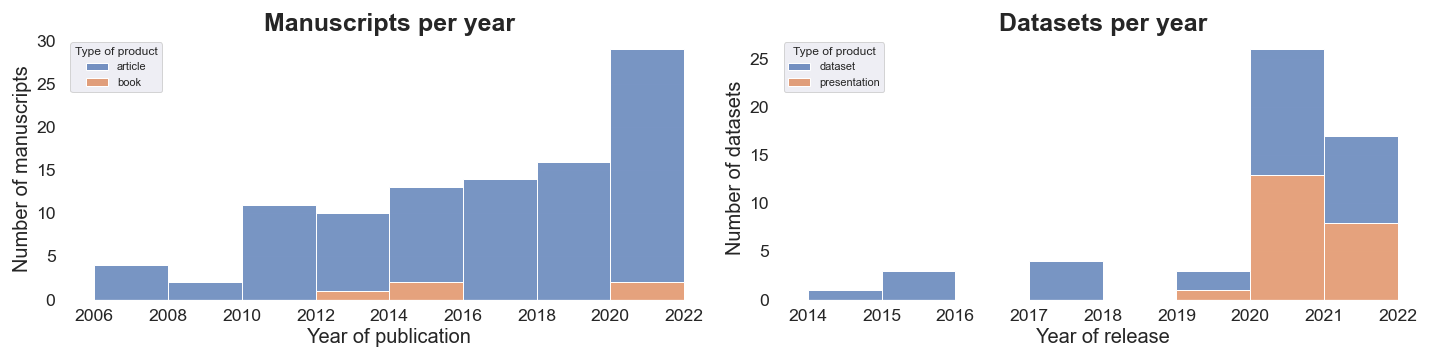
\includegraphics[width=\textwidth]{img/products_per_year.png}
\end{figure}

{\normalfont In the majority of my publications in peer-reviewed international journals, I am listed either as the \textbf{first or last} (senior) author, indicating my primary role in the research and mentorship within these projects. My name is prominently positioned on the author lists, underscoring my substantial contributions. Many papers were \textbf{led or co-authored by students or postdoctoral researchers} whom I have mentored, highlighting my commitment to developing the next generation of scientists.}

\begin{figure}[h]
\centering
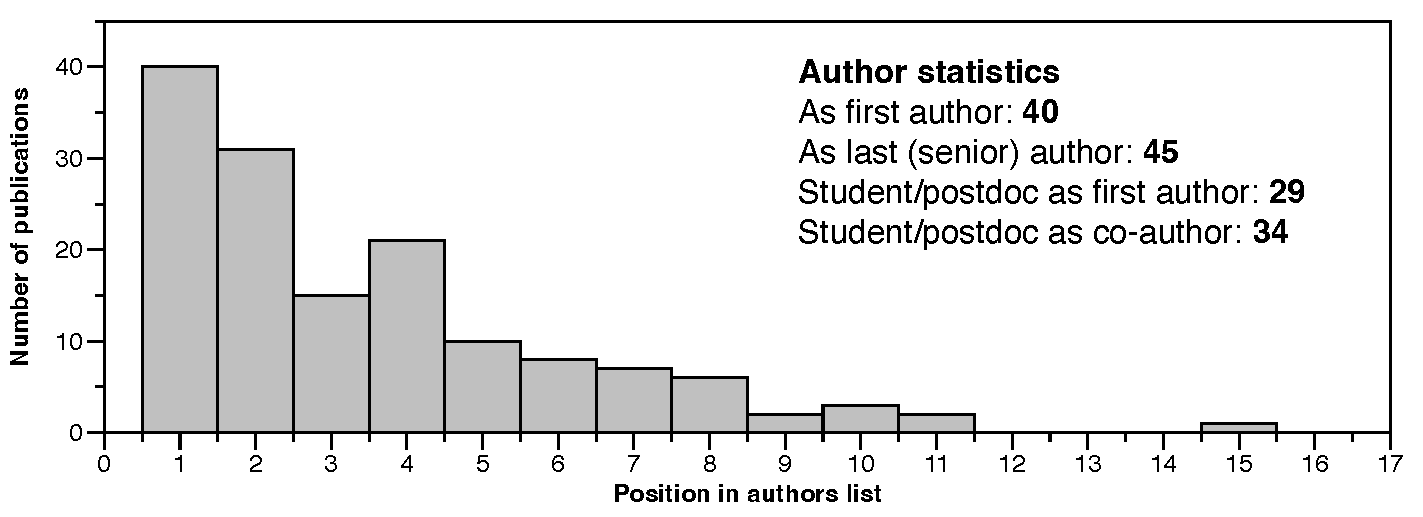
\includegraphics[width=\textwidth]{img/Manuscripts.pdf}
\end{figure}

{\normalfont I have \textbf{107 documents} listed on Scopus, accruing \textbf{4,253 citations} with an \textbf{h-index of 38}. These metrics are somewhat higher on Google Scholar, which accounts for a broader array of research products. On Web of Science, my metrics are dispersed across several automatically generated profiles, potentially affecting the precision of citation counts and other indicators.}

\begin{figure}[h]
\centering
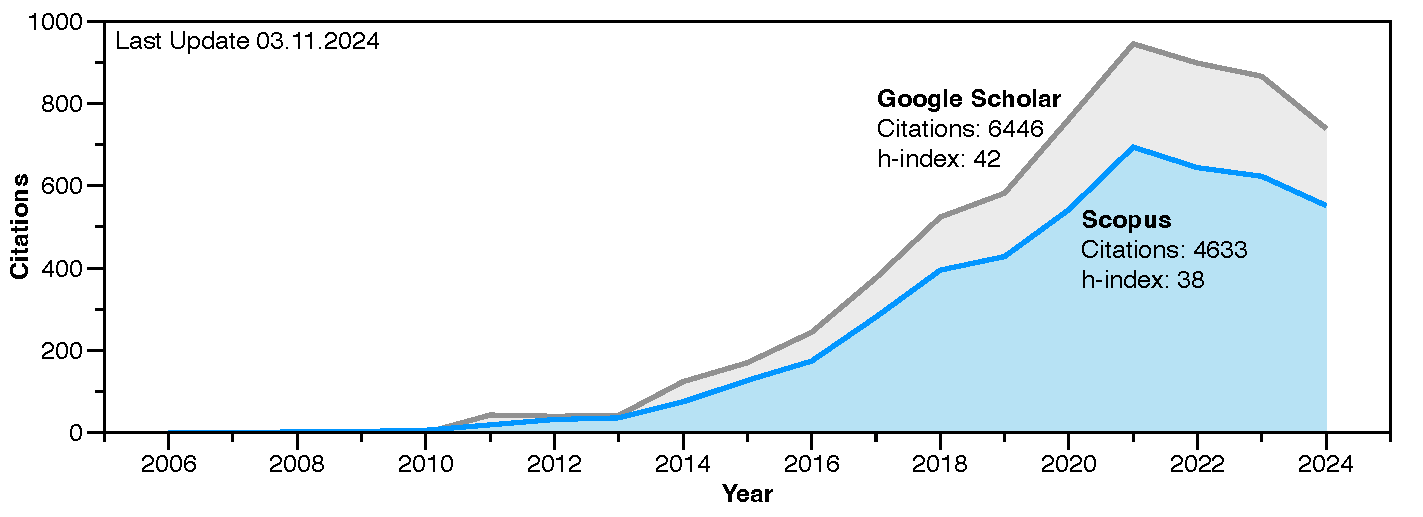
\includegraphics[width=\textwidth]{img/CITATIONS.pdf}
\end{figure}

\newpage

{\normalfont Most of the papers I have co-authored were published in journals \textbf{classified as Q1} by the Journal Citation Reports 2022 (Web of Science), indicating their high impact and prestige within the academic community. My scientific output spans a variety of journals, ranging from sector-specific publications with impact factors between 1 and 5, to \textbf{high-impact journals featuring impact factors greater than 10}, according to the Journal Citation Reports 2022.}

\begin{figure}[h]
\centering
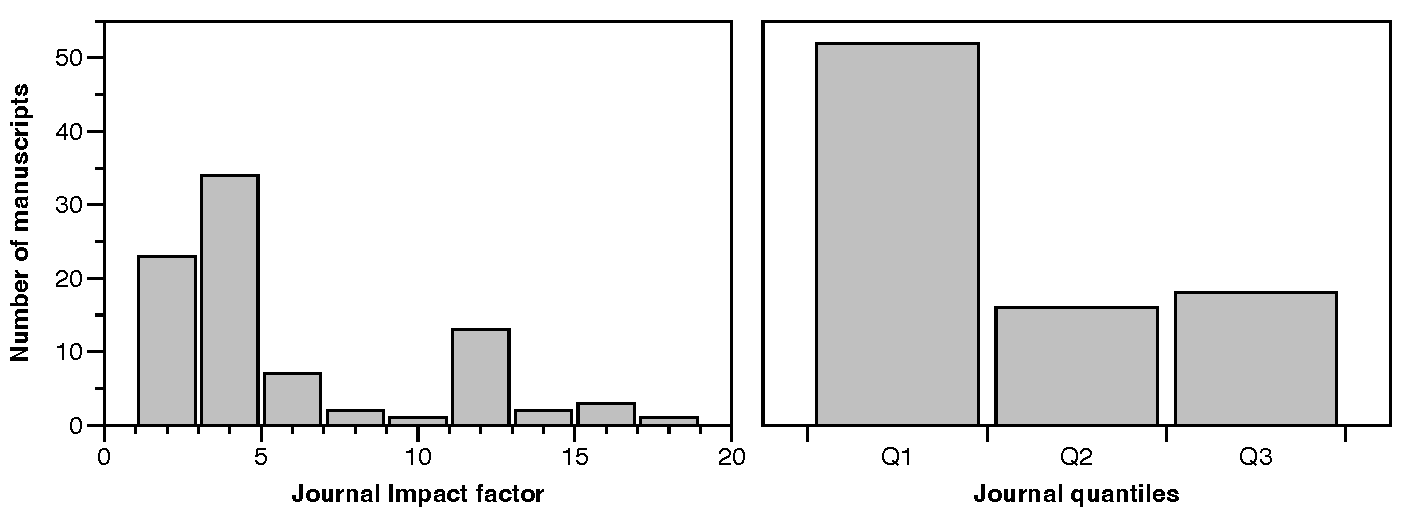
\includegraphics[width=\textwidth]{img/Quantiles.pdf}
\end{figure}

{\normalfont The journals in which I publish primarily fall within the categories of \textbf{physical geography and geosciences}. Additionally, I have published in closely related fields such as ecology and biology, or remote sensing, demonstrating a broad engagement with interdisciplinary research areas.}

\begin{figure}[h]
\centering
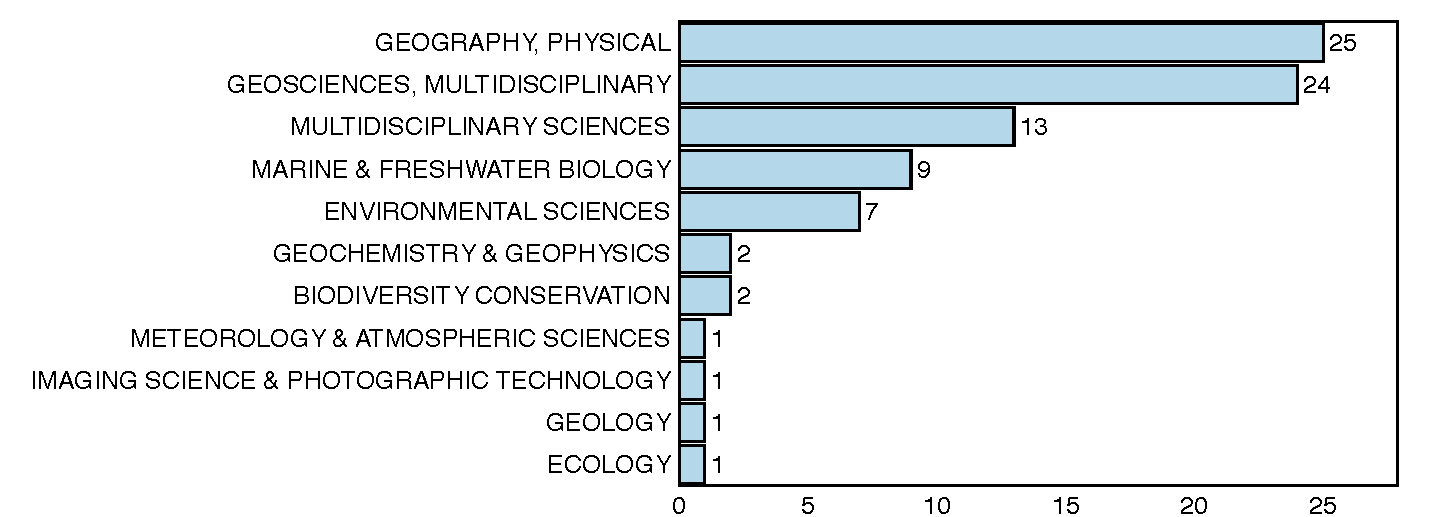
\includegraphics[width=\textwidth]{img/topics.pdf}
\end{figure}
\newpage
{\normalfont An overview of the impact of my research activities from 2013 to 2022 is available from SciVal, a platform developed by Elsevier for analyzing bibliometric research output. According to SciVal, my research during this period encompasses 74 outputs, which have accumulated a total of 3,493 citations. Below are some \textbf{key statistics extracted from SciVal for the years 2013 to 2022.}}
\smallskip

{\footnotesize 
\begin{description}
  \item [39.2\%] of my publications are within the top 10\% most cited worldwide.
  \item [66.7\%] of my publications rank in the top 10\% of journals by CiteScore.
  \item [Q1] 88.4\% of my publications appear in journals classified as Q1 by CiteScore, with the remainder in Q2 journals.
  \item [2.70] is my average Field-Weighted Citation Impact (FWCI). This metric indicates that my publications receive 170\% more citations than the global average for similar works.
\end{description}}

\section{Geographical research focus}
{\normalfont My research spans a broad range of geographical areas, focusing on coastal and sea-level changes. I investigate modern coastal transformations in Germany and Ghana. In tropical areas like Moorea, Tahiti, and Fiji, my studies explore the interactions between modern coastal processes and coral reef ecological dynamics. Additionally, I examine paleo sea-level variations (from the Holocene to the Pliocene) in diverse locations such as the Mediterranean, Cape Verde, the Bahamas, Aruba, Curaçao, Bonaire, Madagascar, Bermuda, Argentina, Brazil, Seychelles, South Africa, and Indonesia. My work also entails studying the underwater topography of coral reefs in the Maldives and ancient sea-level changes on the US East Coast during the Pliocene and Pleistocene epochs. I employ a variety of methodologies to tackle the complexities of marine and coastal geomorphology at these globally distributed sites. I have led research expeditions to all the aforementioned locations, overseeing logistics, securing research permits, and orchestrating the scientific organization of the fieldwork on multiple occasions.}


\begin{figure}[h]
\centering
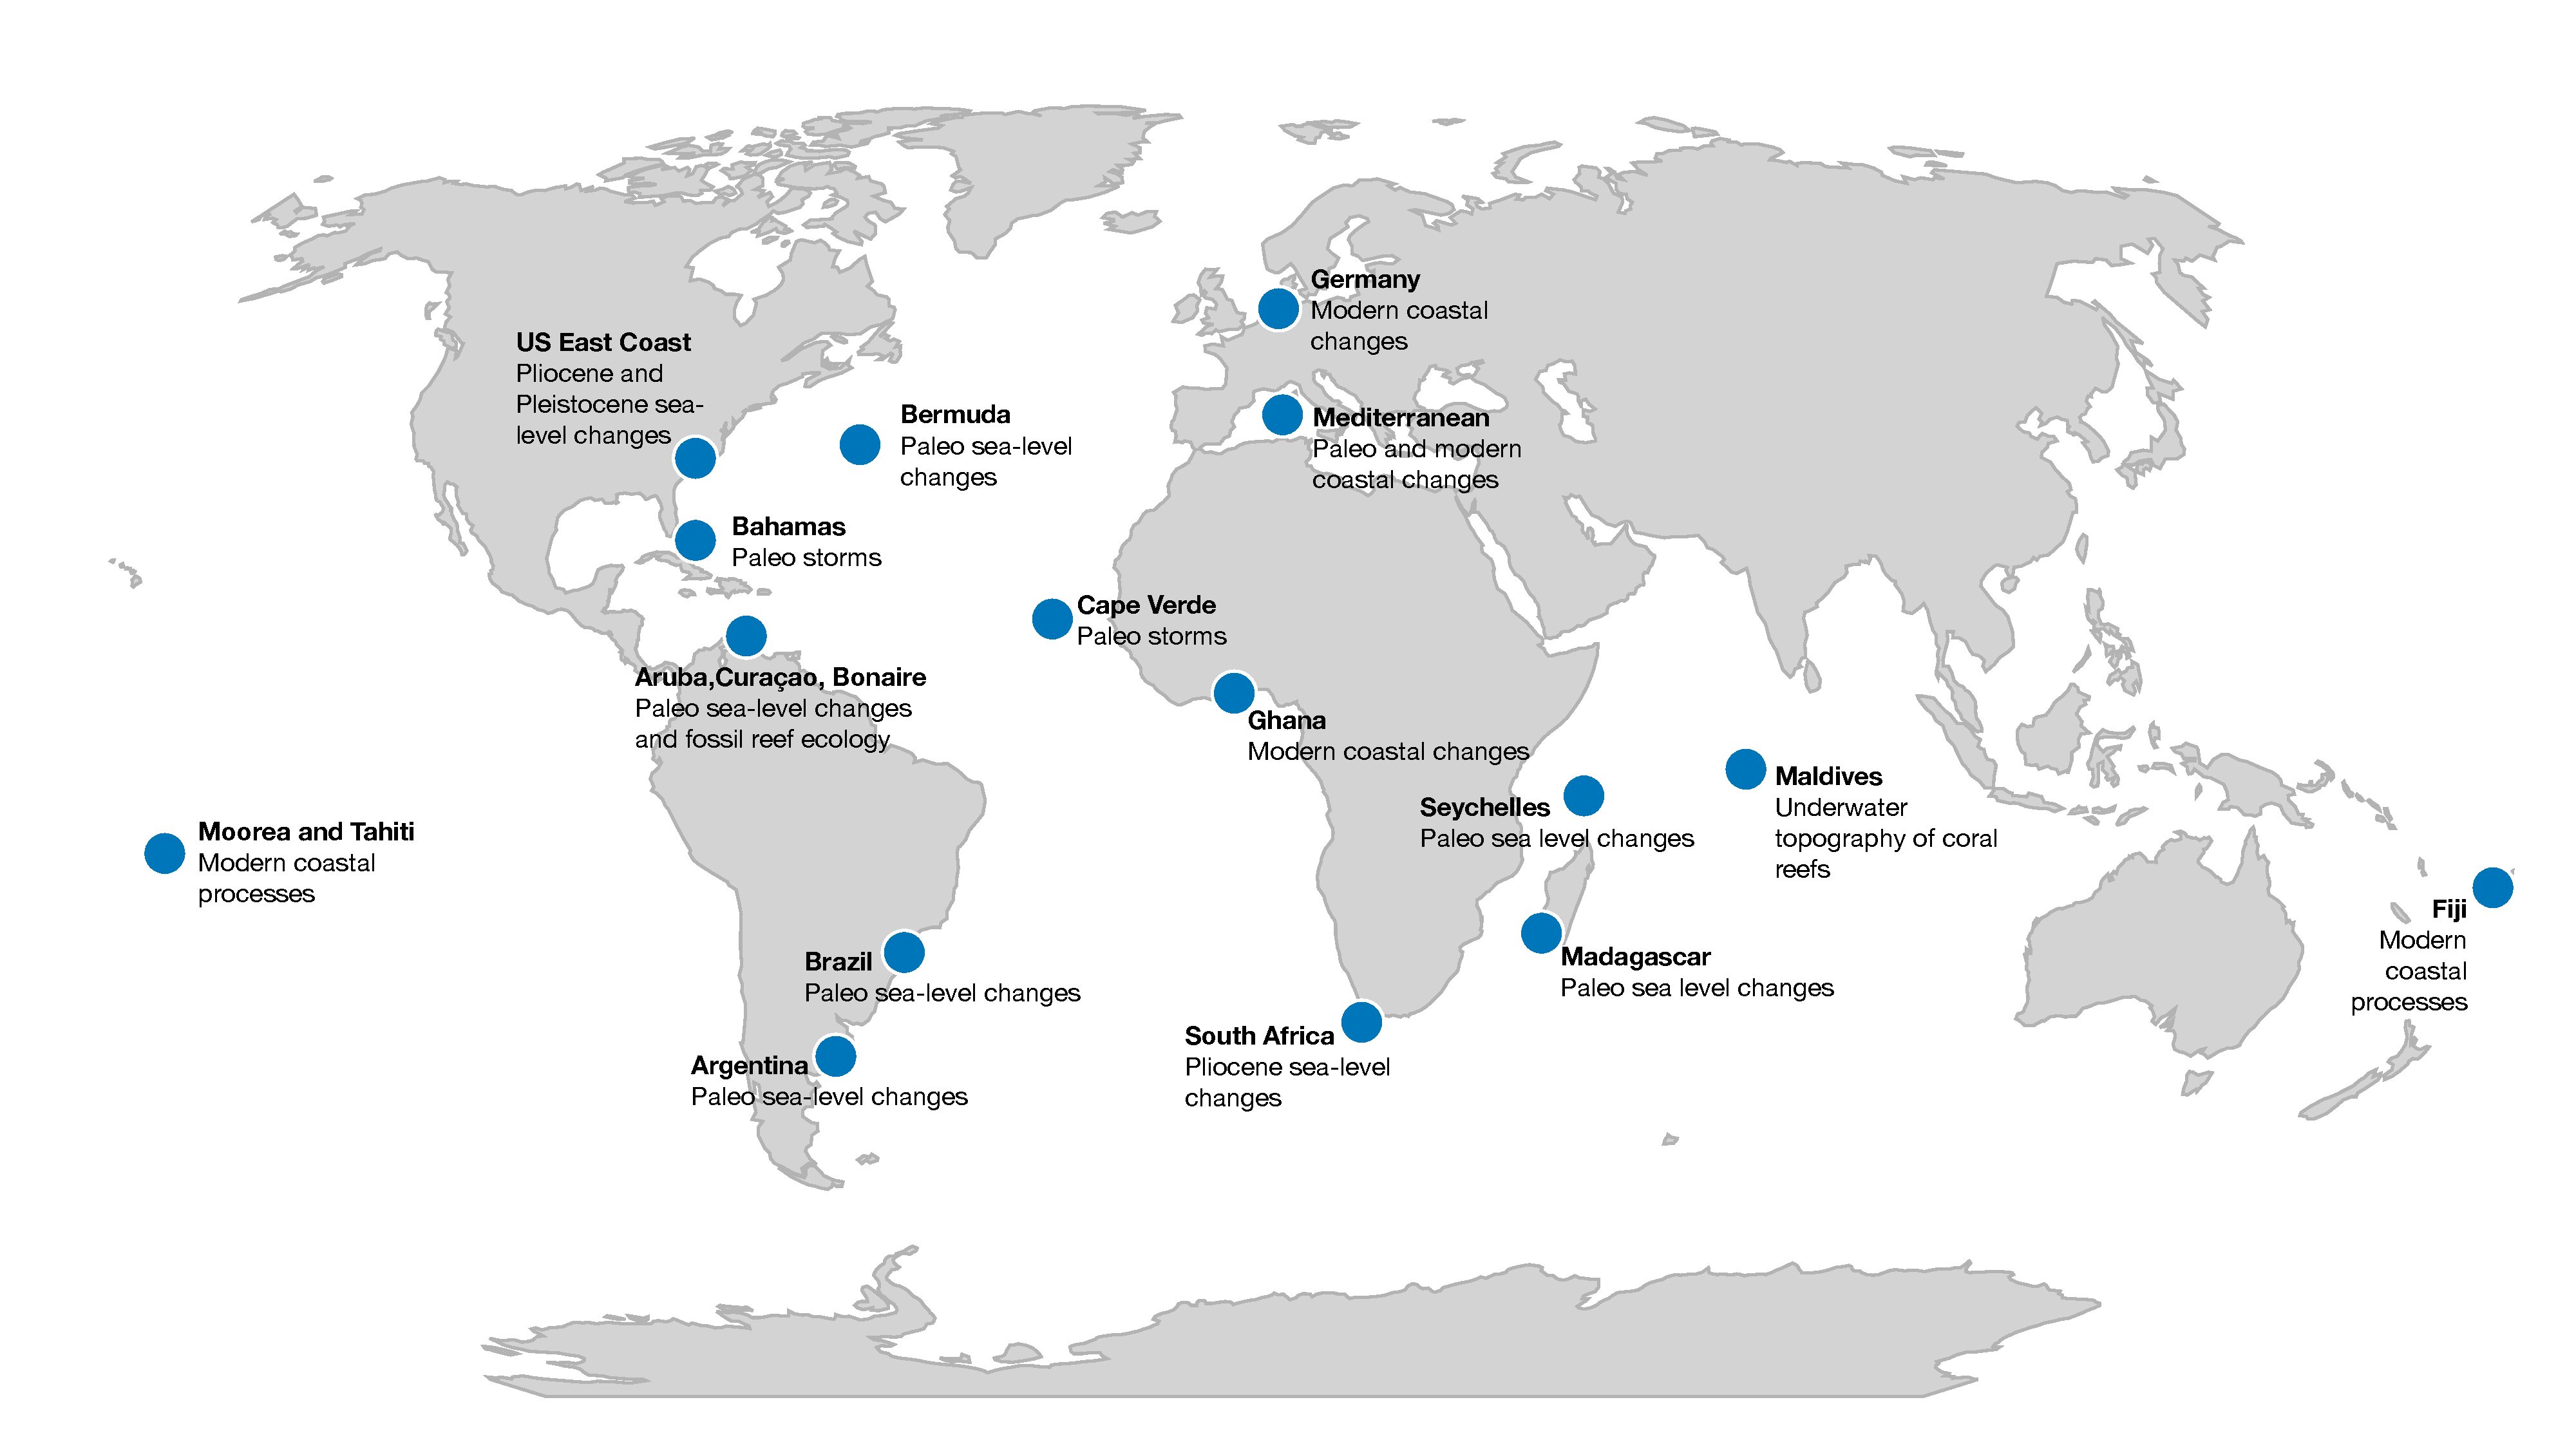
\includegraphics[width=\textwidth]{Research_map/field_data.pdf}
\end{figure}

\newpage
\section{Media reports}
{\normalfont My research activities have been featured in numerous media outlets, including newspapers, radio stations, television channels, and websites. Below, I provide a summary of the principal media reports covering my work.}\\
{\footnotesize 
\begin{description}
  \item [2023] "Ancient warning of a rising sea" (Washington Post, Press, International)
  \item [2023] "Il livello del mare sta salendo. E le nostre coste sono a rischio" (Domani, Press, National) 
  \item [2023] "Ambiente, lo studio: "Livello mare nel 2100 fino a un metro in più rispetto a oggi" (Sky Tg 24, Web Press, National) 
   \item [2023] "Cambiamento climatico e gas serra, nel 2100 il livello del mare può aumentare di un metro: laguna di Venezia sorvegliata speciale" (Il Gazzettino, Web Press, National) 
  \item [2023] "Il nuovo report sul cambiamento climatico: Il mare invaderà certamente le coste, ma possiamo agire per rallentare il fenomeno" (La Stampa, Press, National) 
  \item [2023] "Aruba’s Bocas: home to the rarest fossil reefs on the planet!" (Aruba today, Web Press, International) 
  \item [2022] "Se sparisse il ghiaccio dei Poli..." (Focus, Press, National) 
  \item [2021] "Surprisingly fast ice-melts in past raise fears about sea level rise" (Horizon Magazine, Web Press, National) 
  \item [2021] "E se il mare del passato fosse stato più basso di quanto crediamo?" (Oggiscienza, Press, National) 
  \item [2020] "La sfida delle inondazioni, sempre più violente e frequenti" (Le Scienze, Press, National) 
  \item [2020] "South African seas up to 30m higher show a wet planet under siege" (Daily Maverick, Press, International) 
  \item [2020] "Sea-level rise projections can improve with state-of-the-art model" (Science Daily, Press, International) 
  \item [2017] "Ancient storms could have hurled huge boulders, scientists say" (Washington post, Press, International) 
  \item [2017] "Drohnen liefern detailreiche Einblicke in Korallenriffe" (Der Standard, Press, International) 
  \item [2017] "Mit Drohnen über dem Korallenriff" (Deutschland Radio, Radio, International) 
  \item [2017] "Riffe schützen Inseln vor Monsterwellen. Die Welle" (Die Welle, Web press, International) 
  \item [2017] "Drohnen für die Wissenschaft" (Arte TV, Television, International) 
  \item [2017] "Mit Drohnen gegen die Korallenbleiche" (Welt, Television, International) 
  \item [2016] "I droni contro l’erosione delle coste" (Dronezine, Press, National) 
  \item [2015] "Quatre chercheurs au milieu des surfeurs" (La Depeche de Tahiti, Press, International) 
  \item [2013] "Il business che spinge la startup é l’ecosistema costiero" (Il Secolo XIX, Press, National) 
  \item [2013] "How High Could the Tide Go?" (New York Times, Press, International) 
  \item [2011] "I protagonisti della ricerca scientifica in mare si raccontano" (SubAqua magazine, Press, National) 
\end{description}}

\section{Outreach}
{\normalfont I am actively involved in disseminating my scientific work through content creation on social media channels, with a focus on enhancing science communication. For example, a recent video featuring my expertise produced by Ca' Foscari has garnered approximately 67,000 views on TikTok and 29,000 on Instagram.}\\

\bigskip

\subsection{YouTube $|$ {\normalfont\textit{@CoastalScience}}}
{\footnotesize I create and share videos covering field techniques, geographic information systems, and daily routines in fieldwork. My channel currently has 395 subscribers, and my videos have amassed about 52,000 views, with a total watch time of nearly 3,000 hours.}
\bigskip

\subsection{Podcast $|$ {\normalfont\textit{Storie di Mare}}}
{\footnotesize I produce and host a podcast titled "Storie di Mare," which utilizes storytelling to educate listeners about coastal and marine processes. My episodes have collectively been streamed approximately 2,400 times, and are available on platforms like Spotify, YouTube, and Amazon Music.}
\bigskip

\subsection{Environmental Education $|$ {\normalfont\textit{Sons of the Ocean}}}
{\footnotesize I collaborate with "Sons of the Ocean," a non-profit organization dedicated to environmental education for school-aged children and youth. I contribute media content, including video commentaries for social media, and give presentations aimed at science outreach.}
\bigskip

\newpage
\begin{center}
    {\fontsize{36}{36}\selectfont\interheavy Publications \interthin List} \\ \bigskip
    {\fontsize{14}{14}\selectfont\interthin Publications list - Lista delle pubblicazioni}\\ \bigskip
        {\color{icnclr}} {Names of postdocs, Ph.D. students and master students \\ under my supervision while the article was published are \underline{underlined}}

\end{center}

\nocite{*}
\section{Books and Book chapters}
\printbibliography[type=book,heading=none]

\section{Articles in international journals}
\printbibliography[type=article,heading=none]

\section{Other peer-reviewed articles}
\printbibliography[type=periodical,heading=none]

\section{Open-access datasets}
\printbibliography[type=dataset,heading=none]

\section{Selected presentations}
\printbibliography[type=misc,heading=none]


\end{document}